\chapter{Performance scaling}
\label{c:performance-scaling}
We measure both strong and weak scalings of $\textsc{gamer-sr}$ with AMR and hybrid MPI/OpenMP/GPU
parallelization. The simulations were conducted on the \texttt{Piz-Daint} supercomputer that provides a 12-core Intel Xeon E5-2690 CPU and a Tesla P100 GPU on each computing node. Strong and weak scalings are defined as how the simulation wall time varies with the number of computing nodes for a fixed total problem size and for a fixed problem size per node, respectively. We launch one MPI process with 12 OpenMP threads per node and enable GPU acceleration with single precision.

We divide this section into two parts. First, we measure the strong scaling of a relativistic jet simulation. The simulation set-up, such as initial condition, boundary condition, and grid refinement, follows those described in Section \ref{Limb-brightened jet}. Second, we present the weak scaling for periodic and spherical multi-blast waves test (see \Cref{fig:multi-blast waves}). Note that the overall performance (i.e. total cell updates per second) in both tests have excluded ghost zones in the cell number counts.


    \emph{(1) Strong scaling:}\\
    \Cref{fig:strong scaling} shows the strong scaling results. The parallel efficiency for strong scaling is defined by $\left[T\left(N_{\text{ref}}\right)/T\left(N_{\text{node}}\right)\right]/\left(N_{\text{node}}/N_{\text{ref}}\right)$, where  $T(N_{\text{node}})$ is the simulation wall time using $N_{\text{node}}$ nodes. $N_{\text{ref}}$ is the number of nodes for reference and is fixed to 16 in our test. The overall performance reaches $5\times 10^{10}$ cell updates per second with 2048 GPU nodes, corresponding to a parallel efficiency of $\sim$ 45 per cent. The deviation from the ideal scaling is mainly due to MPI communication as (1) the load-imbalance in the EoS iteration is found to be only subdominant, and (2) the MPI communication time accounts for 45 per cent of the wall time with 2048 nodes. Thus, the parallel efficiency would increase from 0.45 to $0.45/(1-45\%)\sim 0.82$ if excluding MPI communication.

\begin{figure}
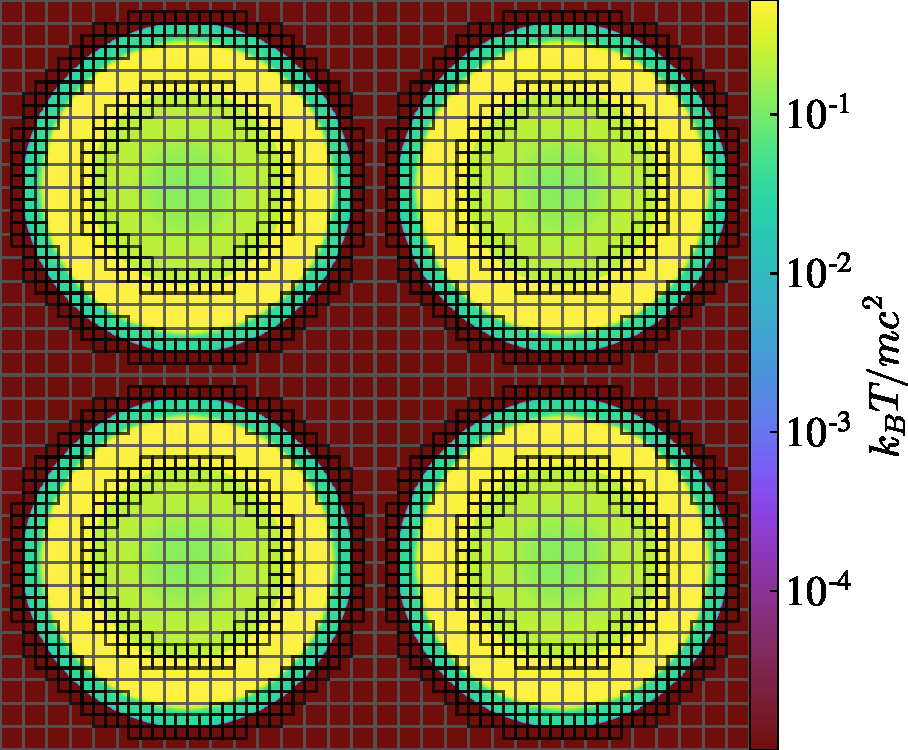
\includegraphics[width=\columnwidth]{figures/fig__weak_scaling.pdf}
\centering
\caption{Temperature slice through the centre of blast waves at $t=0.5L/c$, with the grid patches overlaid in the case of 8 nodes in the weak scaling test.}
\label{fig:multi-blast waves}
\end{figure}

\begin{figure}
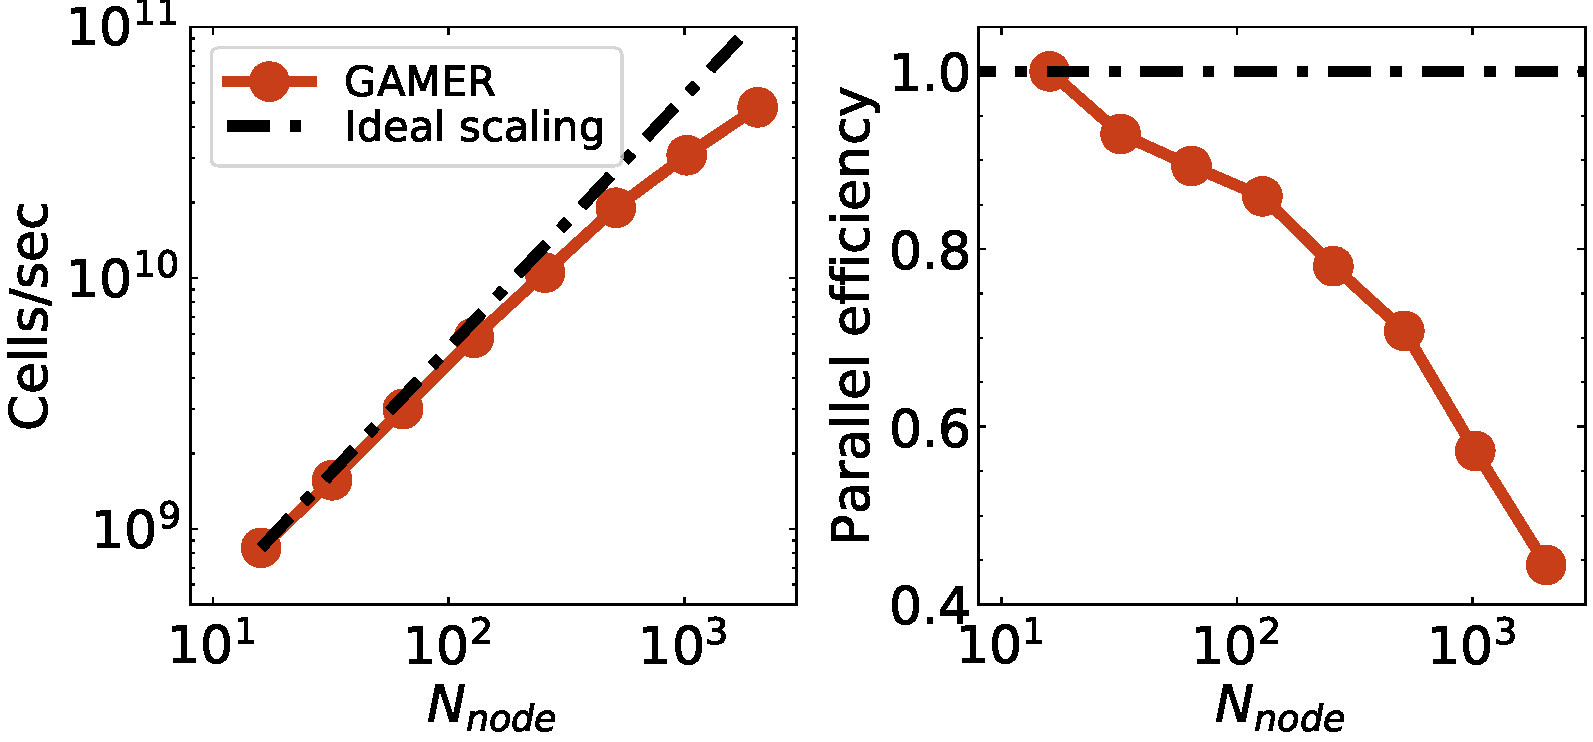
\includegraphics[width=\columnwidth]{figures/fig__benchmark_strongscaling.pdf}
\caption{Strong scaling of the relativistic jet simulation with five AMR levels and 16--2048 GPU nodes (left panel: cell updates per second; right panel: parallel efficiency). The maximum total number of cells, excluding ghost cells, is $7.9\times 10^{9}$. The deviation from the ideal scaling is mainly due to MPI communication, the time fraction of which increases by a factor of 10 when increasing the number of nodes from 64 to 2048.}
\label{fig:strong scaling}
\end{figure}

    \emph{(2) Weak scaling:}\\
    The periodic computational domain is composed of identical cubic subdomain, each of which has a volume of $L^3$ and has an explosion source at its own centre with a radius of $r_{\text{src}}=0.4L$ and an ultra-relativistic temperature of $k_{B}T_{\text{src}}/mc^2=10^{5}$. The uniform ambient gas has a non-relativistic temperature of $k_{B}T_{\text{amb}}/mc^2=10^{-5}$ and a density of $\rho_{\text{src}}=\rho_{\text{amb}}=1.0$. Each subdomain is composed of a $64^3$ base-level grid with three refinement levels, where we refine patches based on the gradient of the reduced energy density. All blast waves evolve from $t=0$ to $t=0.5L/c$. We measure the overall performance and parallel efficiency using $1-2048$ nodes, where each node computes one subdomain. \Cref{fig:multi-blast waves} shows a temperature slice ($z=1.5L$) through the centre of four blast waves at $t=0.5L/c$, with the grid patches overlaid.

\Cref{fig:weak scaling} shows the weak scaling results. The parallel efficiency for weak scaling is defined by $T(1)/T(N_{\text{node}})$, where $T(N_{\text{node}})$ is defined the same as the strong scaling. The parallel efficiency is measured to be 90 per cent with 64 nodes and 78 per cent with 2048 nodes, achieving a peak overall performance of $1.3\times 10^{11}$ cell updates per second with 2048 nodes. The drop of parallel efficiency is mainly due to MPI communication, the time fraction of which increases from 10.3 ($N_{\text{node}}=64$) to 18.8 per cent ($N_{\text{node}}=2048$).

We remark that the strong and weak scaling tests demonstrate 55 and 80 per cent parallel efficiencies, respectively, with 1024 nodes on the \texttt{Piz-Daint} supercomputer. Moreover, the peak performance on a single Tesla P100 GPU achieves $7\times 10^{7}$ cell updates per second, which is about one-third of the peak performance of non-relativistic hydrodynamics \citep{gamer-2}.


\begin{figure}
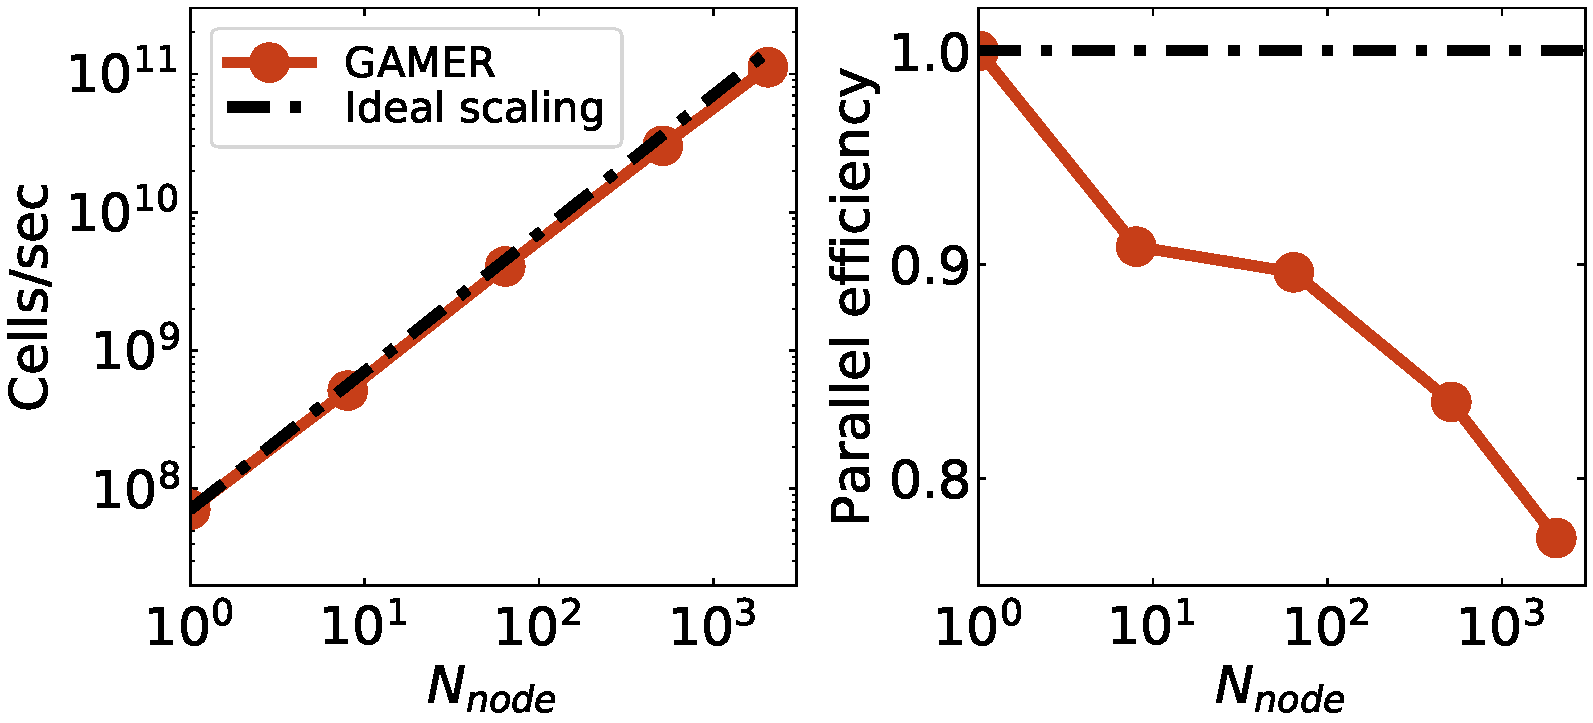
\includegraphics[width=\columnwidth]{figures/fig__benchmark_weakscaling.pdf}
\caption{Weak scaling of the multi-blast waves simulation with three AMR levels and 1--2048 GPU nodes (left panel: cell updates per second; right panel: parallel efficiency). The maximum total number of cells, excluding ghost cells, is $6.9\times 10^{7}$ per node. The parallel efficiency drops from 0.90 to 0.78 when $N_{\text{node}}$ increases from 64 to 2048 mainly because the MPI communication time fraction increases from 10.3 to 18.8 per cent.}
\label{fig:weak scaling}
\end{figure}


\definecolor{BlastSphOld}{RGB}{88, 64, 230}
\definecolor{BlastTriOld}{RGB}{219, 186, 0}
\definecolor{BlastSphNew}{RGB}{199, 62, 24}
\definecolor{BlastTriNew}{RGB}{59, 173, 130}



